\documentclass[11pt,a4paper]{article}
\usepackage{mathpazo}
\usepackage{verbatim}

\usepackage{tikz}
\usetikzlibrary{intersections,calc,through,arrows.meta}
\tikzset {>=Stealth}

\usepackage{url}

\textwidth=15cm
\textheight=23cm
\topmargin=0pt
\headheight=0pt
\oddsidemargin=2em
\headsep=0pt
\parindent=0pt
\renewcommand{\baselinestretch}{1.15}
\setlength{\parskip}{0.3\baselineskip plus 1pt minus 1pt}

\newenvironment{form}[1]{%
\begin{displaymath}%
\renewcommand{\arraystretch}{#1}%
\begin{array}{lcl}}%
{\end{array}%
\end{displaymath}%
}

\newcommand*{\disfrac}[2]{\displaystyle\frac{#1}{#2}}
\newcommand*{\sm}[1]{$\scriptstyle #1$}

\renewcommand*{\floatpagefraction}{.9}
\setlength{\textfloatsep}{10pt plus 2pt minus 4pt}
\setlength{\floatsep}{6pt plus 2pt minus 4pt}

\newcommand*{\occ}[2]{%
  \stackrel{%
    \textstyle r^{#1}}%
    {\!\!\!\scriptscriptstyle #2}}

\begin{document}

%\begin{comment}

\thispagestyle{empty}
\begin{center}
\textbf{\LARGE Construction of a Regular Heptadecagon}

\bigskip

\textbf{\Large Moti Ben-Ari\\\bigskip\url{http://www.weizmann.ac.il/sci-tea/benari/}}

\smallskip

Version 1.0

\medskip
\end{center}


\begin{footnotesize}
\begin{center}
\copyright{}\  2020 by Moti Ben-Ari. 
\end{center}
This work is licensed under the Creative Commons Attribution-ShareAlike 3.0 Unported License. To view a copy of this license, visit \url{http://creativecommons.org/licenses/by-sa/3.0/} or send a letter to Creative Commons, 444 Castro Street, Suite 900, Mountain View, California, 94041, USA.

\end{footnotesize}

This document presents Gauss's insight that it is possible to construct a \emph{heptadecagon}---a regular polygon with $17$ sides---using a straightedge and compass. The presentation is based upon \cite{jorg}; I have added the detailed calculations leading to Gauss's formula. An actual construction from \cite{callagy} is also presented; again I have added the detailed calculations.

\section{Construction of regular polygons}

\paragraph{History}
The ancient Greeks knew how to construct some regular polygons using a straightedge and compass: a triangle, a square, a pentagon and a regular polygon with $15$ sides. Of course, given a regular polygon with $n$ sides, it is easy to construct a polygon with $2n$ sides by bisecting the sides.

No progress was made for two thousand years until in 1796, just before his $19$th birthday, Carl Friedrich Gauss awoke one morning and by ``concentrated thought'' figured out how to construct a regular \emph{heptadecagon}, a regular polygon with $17$ sides. This achievement inspired him to become a mathematician.

The construction of the regular heptadecagon led to the Gauss-Wantzel Theorem which states that a regular polygon with $n$ sides can be constructed using a straightedge and compass if and only if $n$ is the product of a power of $2$ and zero or more \emph{distinct} prime Fermat numbers $2^{2^k}+1$. The known Fermat primes are $F_0=3, F_1=5, F_2=17, F_3=257, F_4=65537$. A regular polygon with $257$ sides was first constructed by Magnus Georg Paucker in $1822$ and Friedrich Julius Richelot $1832$. In $1894$ Johann Gustav Hermes claimed to have constructed a regular polygon  with $65537$ sides and his manuscript is saved at the University of G\"{o}ttigen should you wish to check it.

\paragraph{The cosine of the central angle}
To construct a regular polygon, it is sufficient to construct a line segment of length $\cos \theta$, where $\theta$ is the central angle subtended by a chord that is a side of the polygon inscribed in a unit circle (Figure~\ref{fig.cosine}). Given the line segment $\overline{OB}=\cos\theta$, construct a perpendicular at $B$ and label its intersection with the unit circle by $C$. Then $\cos \theta=\disfrac{\overline{OB}}{\overline{OC}}=\overline{OB}$ so $\theta = \cos^{-1} (\overline{OB})$. The chord $\overline{AC}$ is a side of the polygon.
\begin{figure}
\begin{center}
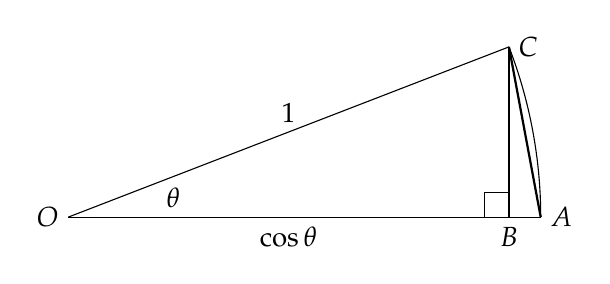
\begin{tikzpicture}[scale=1.5]
\coordinate (O) at (0,0) node[left] {$O$} node[above right,xshift=32pt] {$\theta$};
% {$\cos^{-1} (\cos 21.12^\circ)$};
\coordinate (A) at (4,0);
\node[right] at (A) {$A$};
\draw (O) -- (A);
\draw (A) arc(0:21.12:4);
\coordinate (C) at (21.12:4cm);
\draw (O) -- node[above] {$1$} (C);
\node[right] at (C) {$C$};
\draw (C) -- (C |- A) coordinate (B);
\node[below] at (B) {$B$};
\draw[rotate=90] (B) rectangle +(6pt,6pt);
\draw[thick] (A) -- (C);
\path (O) -- node[below] {$\cos \theta$} (B); % {$\cos 21.12^\circ$} (B);
\end{tikzpicture}
\caption{Constructing a side from the cosine of the central angle it subtends}\label{fig.cosine}
\end{center}
\end{figure}

\paragraph{Constructible lengths} Given a line segment defined to have length $1$, the lengths that are constructible are those which can be obtained from line segments of known length using the operations $\{+,-,\times,\div,\surd\}$.
In Appendices~\ref{a.triangle}, \ref{a.pentagon} we show that a equilateral triangle and a regular pentagon are constructible by giving expressions for  $\cos\left(\disfrac{2\pi}{3}\right)$ and $\cos\left(\disfrac{2\pi}{5}\right)$ that use only the operations $\{+,-,\times,\div,\surd\}$.

\paragraph{Construction of a heptadecagon}
The central angle of a heptadecagon  (Figure~\ref{fig.hept}) is $\disfrac{2\pi}{17}$ radians or $\disfrac{360^\circ}{17}\approx 21.12^\circ$. 
\begin{figure}[bt]
\begin{center}
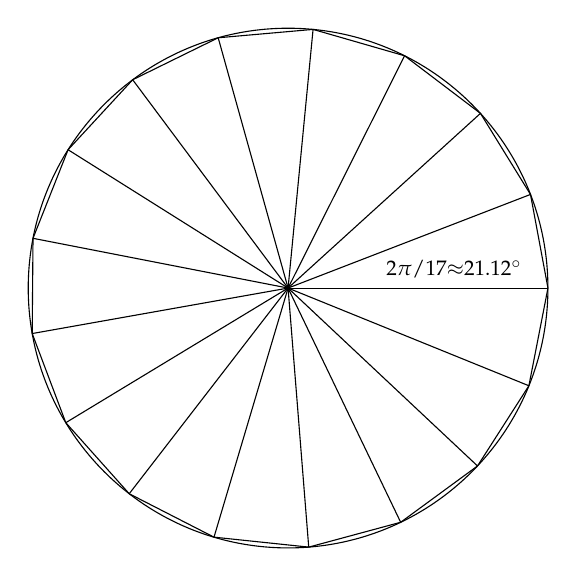
\begin{tikzpicture}[scale=1.1]
\coordinate (O) at (0,0);
\foreach \x/\name in {0/a,1/b,2/c,3/d,4/e,5/f,6/g,7/h,8/i,9/j,10/k,11/l,12/m,13/n,14/o,15/p,16/q} {
  \coordinate (\name) at ($(O)+(\x*21.12:3cm)$);
  \draw (O) -- (\name);
}
\draw (a) -- (b) -- (c) -- (d) -- (e) -- (f) -- (g) -- (h) -- (i) -- (j) -- (k) -- (l) -- (m) -- (n) -- (o) -- (p) -- (q) -- cycle;
\node[above right,xshift=32pt] at (O) {\sm{2\pi/17\approx 21.12^\circ}};
\draw (O) circle (3cm);
\end{tikzpicture}
\caption{A heptadecagon inscribed in a unit circle}\label{fig.hept}
\end{center}
\end{figure}
Gauss showed that \cite{jorg,gauss}:
\begin{form}{3}
\cos\left(\disfrac{2\pi}{17}\right) &=& 
-\disfrac{1}{16}+\disfrac{1}{16}\sqrt{17} + 
     \disfrac{1}{16}\sqrt{34-2\sqrt{17}}
    + \\
    &&
     \disfrac{1}{8}\sqrt{
     17+3\sqrt{17} - 
     \sqrt{34-2\sqrt{17}}
   -2
     \sqrt{34+2\sqrt{17}}
   }\,.
\end{form}
This value can be computed using the operations $\{+,-,\times,\div,\surd\}$ so it is constructible!

Sections~\ref{s.roots}, \ref{s.gauss}, \ref{s.derivation} present Gauss's mathematical ideas, together with the detailed calculations. The proof does not use complex numbers explicitly, though I have added some notes on complex numbers. Section~\ref{s.construction} shows an efficient construction of $\cos\left(\disfrac{2\pi}{17}\right)$.

\section{Roots of unity}\label{s.roots}

We use the following theorem without proof:

\textbf{Fundamental Theorem of Algebra} Every polynomial of degree $n$ (with complex coefficients) has exactly $n$ (complex) roots.

\paragraph{Roots of unity and regular polygons} Consider the equation $x^{n}-1=0$ for any integer $n\geq 1$. One root is $x=1$. By the Fundamental Theorem of Algebra there are $n-1$ other roots. Denote one root by $r$ so that $r^{n}=1$. $r$ is called a \emph{root of unity}.
\begin{center}
\framebox[.9\textwidth]{\parbox{.85\textwidth}{
\textbf{Complex numbers}
The root $r$ is $\cos \left(\disfrac{2\pi}{n}\right) + i\sin  \left(\disfrac{2\pi}{n}\right)$.

By 	de Moivre's formula:
\[
\left[\cos \left(\disfrac{2\pi}{n}\right) + i\sin  \left(\disfrac{2\pi}{n}\right)\right]^{n}=
\cos \left(\disfrac{2\cdot n\pi}{n}\right) + i\sin  \left(\disfrac{2\cdot n\pi}{n}\right)= 1\,.
\]
}}
\end{center}
Consider now $r^2$. Then:
\[
(r^{2})^n=(r^{n})^2=1^2=1\,.
\]
It follows that:
\[
1, r, r^2, \ldots, r^{n-2}, r^{n-1}
\]
are $n$-th roots of unity.

\textbf{Theorem}
Let $n$ be a prime and $r$ an $n$-th root of unity; then $\{1,r,r^2,\ldots,r^{n-2},r^{n-1}\}$ are distinct, so they are \emph{all} the $n$-th roots of unity.

\textbf{Proof} Suppose that $r^i=r^j$ for some $1\leq i<j\leq n$, so $r^j/r^i=r^{j-i}=1$. Let $m$ be the smallest number $0<m<n$ such that $r^m=1$. Now $n=ml+k$ for some $0<l<n$ and $0\leq k<m$. From $1=r^n=r^{ml+k}=(r^m)^l\cdot r^k=1^l\cdot r^k=r^k$, we have $0\leq k<m$ and $r^k=1$. Since $m$ is the smallest such positive integer, $k=0$ and $n=ml$, so $n$ is not prime.

\begin{comment}
\begin{center}
\framebox[.9\textwidth]{\parbox{.85\textwidth}{
\textbf{Complex numbers}
The complex roots are the coordinates of the vertices of a regular polygon inscribed in a unit circle.

For an equilateral triangle, the roots are $1+i\cdot 0,\quad-\disfrac{1}{2}\pm i\disfrac{\sqrt{3}}{2}$.

For a regular pentagon they are:
\[
1+i\cdot 0,\quad\frac{\sqrt{5}-1}{4}\pm i \frac{\sqrt{10+2\sqrt{5}}}{4},\quad\frac{-\sqrt{5}-1}{4}\pm i \frac{\sqrt{10-2\sqrt{5}}}{4}\,.
\]
}}
\end{center}
\end{comment}

We use the following theorem without proof.

\textbf{Theorem} Let $\{a_1,a_2,\ldots,a_{n-1},a_n\}$ be the roots of an $n$-th degree polynomial $f(x)$. Then 
\[
f(x) =(x-a_1) (x-a_2)\cdots (x-a_{n-1})(x-a_n)\,.
\]
Viet\'{e}'s formula \cite[p. 28]{jorg} gives the coefficients of the polynomial in terms of its roots; the formula can be obtained by multiplication. You can see that the coefficient of $x^{n-1}$ is:
\[
-(a_1+a_2+\cdots+a_{n-1}+a_n)\,.
\]
Since the coefficient of $x^{n-1}$ in $x^n-1$ for $n\geq 2$ is obviously zero, we have:
\[
-(1+r+r^2+\cdots + r^{n-2}+r^{n-1})=0\,.
\]
We will use this in the form:
\[
r+r^2+\cdots + r^{n-2}+r^{n-1}=-1\,.
\]
For the heptadecagon this is:
\[
r+r^2+r^3+r^4+r^5+r^6+r^7+r^8+r^9+r^{10}+r^{11}+r^{12}+r^{13}+r^{14} + r^{15}+r^{16}=-1\,.
\]


\section{Gauss's proof that a heptadecagon is constructable}\label{s.gauss}

What Gauss saw is the one need not work with the roots in the natural order $r,r^2,\ldots,r^{16}$. Instead, one can notice that the powers of $r^3$ give all the roots, but in a different order. For $k<17$, $r^{17m+k}=(r^{17})^m\cdot r^k=1^m\cdot r^k=r^k$, so the exponents are reduced modulo $17$:
\begin{form}{1.2}
r^1, \;r^{1\cdot 3 =3},\; r^{3\cdot 3=9},\; r^{9\cdot 3=27=10},\; r^{10\cdot 3=30=13},\; r^{13\cdot 3=39=5},\; r^{5\cdot 3=15},\; r^{15\cdot 3=45=11},&&\\
r^{11\cdot 3 =33=16}, \;r^{16\cdot 3=48=14},\; r^{14\cdot 3=42=8},\; r^{8\cdot 3=24=7},\;r^{7\cdot 3=21=4},\; r^{4\cdot 3=12},\; r^{12\cdot 3=36=2},\; r^{2\cdot 3=6}\,.&&
\end{form}
It is important that you check that this list contains each of the $16$ roots exactly once.

\vspace{-1ex}
\begin{quote}
\textbf{The roots of a quadratic equation} Consider the monic quadratic equation:
\[
y^2+py+q=0\,,
\]
and suppose that its roots are $a,b$. Then:
\[
(y-a)(y-b)=y^2 - (a+b)y + ab\,.
\]
Therefore, $p=-(a+b)$ and $q=ab$, so that if we are \emph{given} $a+b$ and $ab$, we can write down the quadratic equation of which $a,b$ are the roots.\footnote{Po-Shen Lo used this observation to develop a quick method for solving quadratic equations. See \cite{lo}
and a document on my website.}
\end{quote}
\vspace{-1ex}

%We now use this fact on quadratic equations to show that the cosine of the central angle of a heptadecagon can be computed using square roots only.

Let $a_0$ be the sum of the roots in the odd positions in the above list:
\[
a_0=r + r^9 + r^{13} +r^{15} +r^{16} + r^8+r^4+r^2\,,
\]
and let $a_1$ be the sum of the roots in the even positions in the above list:
\[
a_1=r^3 + r^{10} + r^{5} +r^{11} +r^{14} + r^7+r^{12}+r^6\,.
\]
We want to obtain $a_0,a_1$ as roots of a quadratic equation. We first compute their sum:
\[
a_0+a_1=r + r^2 + \cdots +r^{16}=-1\,.
\]

Now we have to work very hard to compute their product! Figure~\ref{fig.a0a1} contains the computation where the values of $r^ir^j$ are written after computing $r^{(i+j) \bmod 17}$. Below each root is its number of occurrences so far; check that each root occurs exactly four times so that the value of the product is $-4$. Since $a_0+a_1=-1$ and $a_0,a_1=-4$, $a_0,a_1$ are the roots of the quadratic equation:
\[
y^2+y-4=0\,,
\]
which are:
\[
a_{0,1} = \frac{-1\pm\sqrt{17}}{2}\,.
\]
\begin{figure}[tb]
\begin{form}{1.5}
a_0a_1&=&(r + r^9 + r^{13} +r^{15} +r^{16} + r^8+r^4+r^2)\;\times\\

&&\quad (r^3 + r^{10} + r^{5} +r^{11} +r^{14} + r^7+r^{12}+r^6)\\

&=&\occ{4}{1} + \occ{11}{1} + \occ{6}{1} + \occ{12}{1} + \occ{15}{1} + \occ{8}{1} + \occ{13}{1} + \occ{7}{1} +\\

&&\occ{12}{2} + \occ{2}{1} + \occ{14}{1} + \occ{3}{1} + \occ{6}{2} + \occ{16}{1} + \occ{4}{2} + \occ{15}{2} +\\

&&\occ{16}{2} + \occ{6}{3} + \occ{1}{1} + \occ{7}{2} + \occ{10}{1} + \occ{3}{2} + \occ{8}{2} + \occ{2}{2}\;\;\: +\\

&&\occ{1}{2} + \occ{8}{3} + \occ{3}{3} + \occ{9}{1} + \occ{12}{3} + \occ{5}{1} + \occ{10}{2} + \occ{4}{3}\;\;\: +\\

&&\occ{2}{3} + \occ{9}{2} + \occ{4}{4} + \occ{10}{3} + \occ{13}{2} + \occ{6}{4} + \occ{11}{2} + \occ{5}{2} \:+\\

&&\occ{11}{3} + \occ{1}{3} + \occ{13}{3} + \occ{2}{4} + \occ{5}{2} + \occ{15}{3} + \occ{3}{4} + \occ{14}{2} \;+\\

&&\occ{7}{3} + \occ{14}{3} + \occ{9}{3} + \occ{15}{4} + \occ{1}{4} + \occ{11}{4} + \occ{16}{3} + \occ{10}{4} +\\

&&\occ{5}{4} + \occ{12}{4} + \occ{7}{4} + \occ{13}{4} + \occ{16}{4} + \occ{9}{4} + \occ{14}{4} + \occ{8}{4}\\
&=&-4\,.
\end{form}\vspace{-2em}
\caption{The computation of $a_0a_1$}\label{fig.a0a1}
\end{figure}
Let $b_0,b_1,b_2,b_3$ be the sum of every fourth root starting with $r^1,r^3,r^9,r^{10}$, respectively:
\begin{form}{1.3}
b_0&=& r^1+ r^{13} + r^{16} + r^4\\
b_1&=& r^3+ r^{5} + r^{14} + r^{12}\\
b_2&=& r^9+ r^{15} + r^{8} + r^2\\
b_3&=& r^{10}+ r^{11} + r^{7} + r^6\,.\\
\end{form}
Check that $b_0+b_2=a_0, b_1+b_3=a_1$. Let us compute the corresponding products:% (Figures~\ref{fig.b0b2}, \ref{fig.b1b3}).
%\begin{figure}[tb]
\begin{form}{1.3}
b_0b_2&=&(r + r^{13} + r^{16} +r^4)\;\times\\
&&\quad (r^9 + r^{15} + r^{8} +r^{2})\\
&=& r^{10}+r^{16}+r^9+r^3+\\
&& r^{5}+r^{11}+r^4+r^{15}+\\
&& r^{8}+r^{14}+r^7+r^1\;\:+\\
&& r^{13}+r^{2}+r^{12}+r^6\\
&=&-1\,,\\
%\vspace{-2em}
%\caption{Computation of $b_0b_2$}\label{fig.b0b2}
%\end{figure}
%\begin{figure}[tb]
%\begin{form}{1.3}
b_1b_3&=&(r^3 + r^{5} + r^{14} +r^{12})\times\\
&&\quad (r^{10} + r^{11} + r^{7} +r^{6})\\
&=& r^{13}+r^{14}+r^{10}+r^9\;+\\
&& r^{15}+r^{16}+r^{12}+r^{11}+\\
&& r^{7}+r^{8}+r^4+r^3\quad\;\;+\\
&& r^{5}+r^{6}+r^{2}+r^1\\
&=&-1\,.
\end{form}
%\vspace{-2em}
%\caption{Computation of $b_1b_3$}\label{fig.b1b3}
%\end{figure}
To summarize these computations:
\begin{form}{1.2}
b_0+b_2&=&a_0\\
b_0b_2&=&-1\\
b_1+b_3&=&a_1\\
b_1b_3&=&-1\,,
\end{form}
so $b_0,b_2$ are the solutions of:
\[
y^2-a_0y-1= 0\,.\\
\]
and $b_1,b_3$ are the solutions of:
\[
y^2-a_1y-1 =0\,.
\]
Using the formula for solving quadratic equations and the values previously computed for $a_0,a_1$, we obtain the roots $b_0,b_1$ (Figure~\ref{fig.b01}).
\begin{figure}
\begin{form}{2.7}
b_0&=&\disfrac{a_0+\sqrt{a_0^2+4}}{2}\\
&=&\disfrac{
     \disfrac{(-1+\sqrt{17})}{2} + 
     \sqrt{\left(\disfrac{(-1+\sqrt{17})}{2}\right)^2+4}
   }{2}\\
&=&\disfrac{
     (-1+\sqrt{17}) + 
     \sqrt{\left(-1+\sqrt{17}\right)^2+16}
   }{4}\\
&=&\disfrac{
     (-1+\sqrt{17}) + 
     \sqrt{34-2\sqrt{17}}
   }{4}\,,\\
%\end{form}%\vspace{-2em}
%\caption{Computation of $b_0$}\label{fig.b0}
%\end{figure}
%\begin{figure}
%\begin{form}{2.8}
b_1&=&\disfrac{a_1+\sqrt{a_1^2+4}}{2}\\
&=&\disfrac{
     \disfrac{(-1-\sqrt{17})}{2} + 
     \sqrt{\left(\disfrac{(-1-\sqrt{17})}{2}\right)^2+4}
   }{2}\\
&=&\disfrac{
     (-1-\sqrt{17}) + 
     \sqrt{\left(-1-\sqrt{17}\right)^2+16}
   }{4}\\
&=&\disfrac{
     (-1-\sqrt{17}) + 
     \sqrt{34+2\sqrt{17}}
   }{4}\,.
\end{form}\vspace{-2em}
\caption{Computation of $b_0,b_1$}\label{fig.b01}
\end{figure}
%\begin{form}{1.4}
%b_1b_3&=&(r^3 + r^{5} + r^{14} +r^{12})\times\\
%&&(r^{10} + r^{11} + r^{7} +r^{6})\\
%&=& r^{13}+r^{14}+r^{10}+r^9\;+\\
%&& r^{15}+r^{16}+r^{12}+r^{11}+\\
%&& r^{7}+r^{8}+r^4+r^3\quad\;\;+\\
%&& r^{5}+r^{6}+r^{2}+r^1\\
%&=&-1\,.
%\end{form}

Finally, let $c_0,c_4$ be the sum of every eighth root starting with $r^1,r^{13}$, respectively:\footnote{There are other sums but these two suffice.}
\begin{form}{1.4}
c_0&=&r^1+r^{16}\\
c_4&=&r^{13}+r^4\\
c_0+c_4&=&r^1+r^{16}+r^{13}+r^4=b_0\\
c_0c_4&=&(r^1+r^{16})\cdot(r^{13}+r^4)\\
&=&r^{14}+r^5+r^{12}+r^3=b_1\,,
\end{form}
so $c_0,c_4$ are the roots of:
\[
y^2-b_0y+b_1=0
\]
It suffices to compute the root $c_0=r^1+r^{16}$
(Figure~\ref{fig.c0}) since:
\[
c_0=r_1+r_{16}=2\cos\left(\frac{2\pi}{17}\right)\,,
\]
as shown in Figure~\ref{fig.two-cosine}. The $y$-coordinates are equal but with opposite signs and cancel, while the $x$-coordinate is counted twice.
Therefore, the cosine of the central angle of a heptadecagon is constructible with straightedge and compass, since it is composed only of rational numbers and the operations $\{+,-,\times,\div,\surd\}$:

\begin{form}{2.2}
\cos\left(\disfrac{2\pi}{17}\right) &=& 
\disfrac{c_0}{2}\\
&=&
-\disfrac{1}{16}+\disfrac{1}{16}\sqrt{17} + 
     \disfrac{1}{16}\sqrt{34-2\sqrt{17}}
    + \\
    &&
     \disfrac{1}{16}\sqrt{
     68+12\sqrt{17} + 
     2(-1+\sqrt{17})\sqrt{34-2\sqrt{17}}
   -16
     \sqrt{34+2\sqrt{17}}
   }
\end{form}

\begin{figure}
\begin{center}
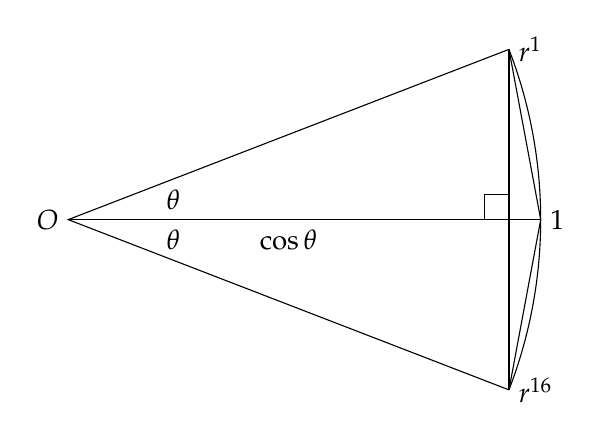
\begin{tikzpicture}[scale=1.5]
\coordinate (O) at (0,0) node[left] {$O$} node[above right,xshift=32pt] {$\theta$} node[below right,xshift=32pt] {$\theta$};
\coordinate (A) at (4,0);
\node[right] at (A) {$1$};
\draw (O) -- (A);
\coordinate (C) at (21.12:4cm);
\coordinate (D) at (-21.12:4cm);
\draw (D) arc(-21.12:21.12:4);
\draw (D) -- (O) -- (C);
\node[right] at (C) {$r^1$};
\node[right] at (D) {$r^{16}$};
\draw (C) -- (C |- A) coordinate (B);
\draw (D) -- (D |- A);
%\node[below left] at (B) {$B$};
\draw[rotate=90] (B) rectangle +(6pt,6pt);
\draw (D) -- (A) -- (C);
\path (O) -- node[below] {$\cos \theta$} (B);
\end{tikzpicture}
\caption{Constructing a side from the cosine of the central angle it subtends}\label{fig.two-cosine}
\end{center}
\end{figure}

\begin{figure}
\begin{form}{2.8}
c_0&=&\disfrac{b_0+\sqrt{b_0^2-4b_1}}{2}\\
&=&\disfrac{
     \disfrac{
     (-1+\sqrt{17}) + 
     \sqrt{34-2\sqrt{17}}
   }{4}}{2} + \\
&& 
    \disfrac{
       \sqrt{\left[\disfrac{
     (-1+\sqrt{17}) + 
     \sqrt{34-2\sqrt{17}}
   }{4}\right]^2-4\left[\disfrac{
     (-1-\sqrt{17}) + 
     \sqrt{34+2\sqrt{17}}
   }{4}\right]}
   }{2}\\
&=&-\disfrac{1}{8}+\disfrac{1}{8}\sqrt{17} + 
     \disfrac{1}{8}\sqrt{34-2\sqrt{17}}
    + \\
   &&
     \disfrac{1}{8}\sqrt{
     \left[
     (-1+\sqrt{17}) + 
     \sqrt{34-2\sqrt{17}}
   \right]^2-16\left[
     (-1-\sqrt{17}) + 
     \sqrt{34+2\sqrt{17}}
   \right]}
\\
&=&-\disfrac{1}{8}+\disfrac{1}{8}\sqrt{17} + 
     \disfrac{1}{8}\sqrt{34-2\sqrt{17}}
    + \\
   &&
     \disfrac{1}{8}\sqrt{
     (-1+\sqrt{17})^2 + 
     2(-1+\sqrt{17})\sqrt{34-2\sqrt{17}}+
     (34-2\sqrt{17})
   -}\\
   &&\overline{
     \left[(-16-16\sqrt{17}) + 
     16\sqrt{34+2\sqrt{17}}\right]
   }
\\
&=&-\disfrac{1}{8}+\disfrac{1}{8}\sqrt{17} + 
     \disfrac{1}{8}\sqrt{34-2\sqrt{17}}
    + \\
   &&
     \disfrac{1}{8}\sqrt{
     68+12\sqrt{17} + 
     2(-1+\sqrt{17})\sqrt{34-2\sqrt{17}}
   -16
     \sqrt{34+2\sqrt{17}}
   }

\end{form}
\caption{Computation of $c_0$}\label{fig.c0}
\end{figure}


\begin{center}
\framebox[.9\textwidth]{\parbox{.85\textwidth}{
\textbf{Complex numbers}
\begin{form}{1.8}
c_0\!\!\!&=&\!\!\!r_1+r_{16}\\
\!\!\!&=&\!\!\!\cos\left(\disfrac{2\pi}{17}\right)\!+i\sin\left(\disfrac{2\pi}{17}\right)+\cos\left(\disfrac{2\cdot 16\pi}{17}\right)\!+i\sin\left(\disfrac{2\cdot 16\pi}{17}\right)\\
\!\!\!&=&\!\!\!\cos\left(\disfrac{2\pi}{17}\right)\!+i\sin\left(\disfrac{2\pi}{17}\right)+\cos\left(\disfrac{-2\pi}{17}\right)\!+i\sin\left(\disfrac{-2\pi}{17}\right)\\
&=&2\cos\left(\disfrac{2\pi}{17}\right)\,.
\end{form}
}}
\end{center}

\clearpage
%\begin{form}{1.2}
%\cos\left(\disfrac{2\pi}{17}\right) &=& 
%-\disfrac{1}{16}+\disfrac{1}{16}\sqrt{17} + 
%     \disfrac{1}{16}\sqrt{34-2\sqrt{17}}
%    + \\
%    &=&
%     \disfrac{1}{16}\sqrt{
%     68+12\sqrt{17} + 
%     2(-1+\sqrt{17})\sqrt{34-2\sqrt{17}}
%   -16
%     \sqrt{34+2\sqrt{17}}
%   }\,.
%\end{form}

\section{Derivation of Gauss's formula}\label{s.derivation}

The formula we gave for $\cos\left(\disfrac{2\pi}{17}\right)$ is not the one given by Gauss \cite[p.~458]{gauss}, which also appears in \cite[p.~68]{jorg}. I found it only in \cite{rike}, where Rike gives it as an exercise to transform the formula to the one that Gauss gave. This Section gives that transformation.

Let us simplify $2(-1+\sqrt{17})\sqrt{34-2\sqrt{17}}$:
\begin{form}{1.7}
2(-1+\sqrt{17})\sqrt{34-2\sqrt{17}} &=&
-2\sqrt{34-2\sqrt{17}} +2\sqrt{17}\sqrt{34-2\sqrt{17}}+\\
&&4\sqrt{34-2\sqrt{17}}-4\sqrt{34-2\sqrt{17}}\\
&=&
2\sqrt{34-2\sqrt{17}} +2\sqrt{17}\sqrt{34-2\sqrt{17}}+\\
&&-4\sqrt{34-2\sqrt{17}}\\
%&=&\left(-2\sqrt{34-2\sqrt{17}} +2\sqrt{17}\sqrt{34-2\sqrt{17}}
%+4\sqrt{34-2\sqrt{17}}\right)\\
%&&-4\sqrt{34-2\sqrt{17}}\\
&=&2(1+\sqrt{17})\sqrt{34-2\sqrt{17}}-4\sqrt{34-2\sqrt{17}}\,.\\
\end{form}
We will remember the term $-4\sqrt{34-2\sqrt{17}}$ for now and simplify the first term by squaring it and then taking the square root:
\begin{form}{1.8}
2(1+\sqrt{17})\sqrt{34-2\sqrt{17}}&=&
2\sqrt{\left[(1+\sqrt{17})\sqrt{34-2\sqrt{17}}\right]^2}\\
&=&2\sqrt{(18+2\sqrt{17})(34-2\sqrt{17})}\\
&=&2\sqrt{(18\cdot 34-4\cdot17)+\sqrt{17}(2\cdot 34 - 2\cdot 18)}\\
&=&2\cdot 4\sqrt{34+2\sqrt{17}}\,.
\end{form}
Substituting terms results in Gauss's formula:
\begin{form}{2.2}
\cos\left(\disfrac{2\pi}{17}\right) &=& 
-\disfrac{1}{16}+\disfrac{1}{16}\sqrt{17} + 
     \disfrac{1}{16}\sqrt{34-2\sqrt{17}}
    + \\
    &&
     \disfrac{1}{16}\sqrt{
     68+12\sqrt{17} + 
     2\cdot 4\sqrt{34+2\sqrt{17}}-4\sqrt{34-2\sqrt{17}}
   -16
     \sqrt{34+2\sqrt{17}}
   }\\
&=&-\disfrac{1}{16}+\frac{1}{16}\sqrt{17} + 
     \disfrac{1}{16}\sqrt{34-2\sqrt{17}}
    + \\
    &&
     \disfrac{1}{8}\sqrt{
     17+3\sqrt{17} - 
     \sqrt{34-2\sqrt{17}}
   -2
     \sqrt{34+2\sqrt{17}}
   }\,.
\end{form}

%Computing the expression with a calculator gives $\cos\left(\disfrac{2\pi}{17}\right)\approx 0.298$ and $\cos^{-1}0.298\approx 0.3699$ radians or $21.2926^\circ$. The correct value is $\disfrac{2\pi}{17}\approx .3696$ radians or $\disfrac{360^\circ}{17}\approx 21.176^\circ$.

\newpage

\section{Construction with a straightedge and compass}\label{s.construction}
Several constructions are given in \cite{wiki:heptadecagon}. Here I give the construction from \cite{callagy} because it directly constructs $\cos\left( \disfrac{2\pi}{17}\right)$. The construction uses only Pythagoras's Theorem and the Angle Bisector Theorem \cite{wiki:bisector}.

Construct a unit circle centered at  $O$,  and construct perpendicular diameters,  $\overline{QP}, \overline{SR}$.\footnote{To save space I have clipped the circle so that $R=(0,1),S=(0,-1)$ do not appear.}
\begin{center}
\begin{tikzpicture}[scale=1.5]
\clip (-5,-1.8) rectangle (5,1.8);

\node at (-.2,1.5) {$\cdots$};
\node at (-.2,1.7) {$R$};
\node at (-.2,-1.5) {$\cdots$};
\node at (-.2,-1.7) {$S$};

\coordinate (O) at (0,0);
\draw (O) circle (4cm);
\coordinate (P) at (4,0);
\coordinate (R) at (0,4);
\coordinate (Q) at (-4,0);
\coordinate (S) at (0,-4);
\coordinate (A) at (0,1);
\coordinate (B) at (.78,0);
\coordinate (C) at (-1.28,0);
\draw (P) -- (Q);
\draw (R) -- (S);
\path (O) -- node[left,xshift=2pt,yshift=-4pt] {\sm{\frac{1}{4}}} (A);
\draw[dashed] (P) -- ($(P)!1.5!(A)$);
\draw (A) -- node[above] {$\frac{\sqrt{17}}{4}$} (P);
\draw (C) -- (A) -- (B);
\foreach \c/\where in {O/below left, P/right, Q/left, R/above, S/below, A/above left, B/below, C/below} {
  \fill (\c) circle(1.5pt) node[\where] {$\c$};
}
\draw (O) rectangle(+6pt,+6pt);
\node[below right,xshift=8pt,yshift=-4pt] at (A) {\sm{\alpha}};
\node[below right,xshift=-3pt,yshift=-4pt] at (A) {\sm{\alpha}};
\node[below left,xshift=1pt,yshift=-2pt] at (A) {\sm{\beta}};
\node[below left,xshift=-4pt,yshift=4pt] at (A) {\sm{\beta}};
\draw[<->] ($(C)+(0,-16pt)$) -- node[below] {\sm{\frac{1+\sqrt{17}}{16}}} ($(O)+(0,-16pt)$);
\draw[<->] ($(O)+(0,-16pt)$) -- node[below,xshift=4pt] {
\sm{
\frac{\sqrt{34+2\sqrt{17}}}{16}
}
} ($(B)+(0,-16pt)$);
\end{tikzpicture}
\end{center}
Construct $A$ so that $\overline{OA}=\disfrac{1}{4}\overline{OR}$. By Pythagoras's Theorem:
\[
\overline{AP}=\sqrt{(1/4)^2+1^2}=\sqrt{17}/4\,.
\]
Let $B$ be the intersection of the internal bisector of $\angle OAP$ and $\overline{OP}$, and let $C$ be the intersection of the external bisector of $\angle OAP$ and $\overline{QO}$. By the angle bisector theorem:
\begin{form}{2}
\disfrac{\overline{OB}}{\overline{BP}}&=&\disfrac{\overline{AO}}{\overline{AP}}\\
\disfrac{\overline{OB}}{1-\overline{OB}}&=&\disfrac{1/4}{\sqrt{17}/{4}}\\
\overline{OB}&=&\disfrac{1}{1+\sqrt{17}}=\disfrac{1}{1+\sqrt{17}}\cdot \disfrac{1-\sqrt{17}}{1-\sqrt{17}}\\
&=&\disfrac{-1+\sqrt{17}}{16}\,,
\end{form}
and:
\begin{form}{2}
\disfrac{\overline{OC}}{\overline{CP}}&=&\disfrac{\overline{AO}}{\overline{AP}}\\
\disfrac{\overline{OC}}{1-\overline{OC}}&=&\disfrac{1/4}{\sqrt{17}/{4}}\\
\overline{OC}&=&\disfrac{1}{-1+\sqrt{17}}=\disfrac{1}{-1+\sqrt{17}}\cdot \disfrac{1+\sqrt{17}}{1+\sqrt{17}}\\
&=&\disfrac{1+\sqrt{17}}{16}\,.
\end{form}

\pagebreak[3]

Construct $D$ on $\overline{OP}$ such that $\overline{CD}=\overline{CA}$:
\begin{center}
\begin{tikzpicture}[scale=1.5]
\clip (-5,-1.5) rectangle (5,1.5);
\coordinate (O) at (0,0);
\draw (O) circle (4cm);
\coordinate (P) at (4,0);
\coordinate (R) at (0,4);
\coordinate (Q) at (-4,0);
\coordinate (S) at (0,-4);
\coordinate (A) at (0,1);
\coordinate (B) at (.78,0);
\coordinate (C) at (-1.28,0);

\coordinate (D) at (.344,0);
\coordinate (E) at (2.05,0);
\coordinate (M) at (-1.8275,0);
\coordinate (F) at (0,-1);

\draw (P) -- (Q);
\draw (R) -- (S);
\draw (A) -- (P);
\draw (C) -- node[above] {$a$} (A) -- node[above] {$b$} (B);
\path (Q) -- node[below] {$f$}  (M);
\path (B) -- node[below] {$b$} (E);

\path[name path=circ] (M) circle (2.1725cm);
\path[name path=yaxis] (R) -- (S);
\path[name intersections={of=circ and yaxis,by={F1,F}}];
\draw (M) -- node[below] {$f$} (F);

\draw[<->] ($(C)+(0,-10pt)$) -- node[fill=white] {$a$} ($(D)+(0,-10pt)$);

\foreach \c/\where in {O/below left, P/right, Q/left, R/above, S/below, A/above left, B/below, C/below, D/below, E/below, M/below left, F/below left} {
  \fill (\c) circle(1pt) node[\where] {$\c$};
}
\draw (O) rectangle(+6pt,+6pt);
\end{tikzpicture}
\end{center}
\begin{form}{2}
\overline{CD}=\overline{CA}&=&\sqrt{\overline{OA}^2+\overline{OC}^2}\\
&=&\sqrt{\left(\disfrac{1}{4}\right)^2+\left(\disfrac{1+\sqrt{17}}{16}\right)^2}\\
&=&\disfrac{1}{16}\sqrt{34+2\sqrt{17}}\,.
\end{form}
Construct $E$ on $\overline{OP}$ such that $\overline{BE}=\overline{BA}$:
\begin{form}{2}
\overline{BE}=\overline{BA}&=&\sqrt{\overline{OA}^2+\overline{OB}^2}\\
&=&\sqrt{\left(\disfrac{1}{4}\right)^2+\left(\disfrac{1-\sqrt{17}}{16}\right)^2}\\
&=&\disfrac{1}{16}\sqrt{34-2\sqrt{17}}\,.
\end{form}
Construct $M$ as the midpoint of $\overline{QD}$ and construct $F$ on $\overline{OS}$ such that $\overline{MF}=\overline{MQ}$:
\begin{form}{2}
\overline{MF}=\overline{MQ}&=&\disfrac{1}{2}\overline{QD}=\disfrac{1}{2}(\overline{QC}+\overline{CD})=\disfrac{1}{2}((1-\overline{OC})+\overline{CD})\\
&=&\disfrac{1}{2}\left[1-\left(\disfrac{1+\sqrt{17}}{16}\right)+\disfrac{\sqrt{34+2\sqrt{17}}}{16}\right]\\
&=&\disfrac{1}{32}\left(15-\sqrt{17}+\sqrt{34+2\sqrt{17}}\right)\,.
\end{form}
Construct a circle whose diameter is $\overline{OE}$. Construct a chord $\overline{OG}=\overline{OF}$. Note that $\overline{MO}=1-\overline{MQ}=1-\overline{MF}$:
\begin{center}
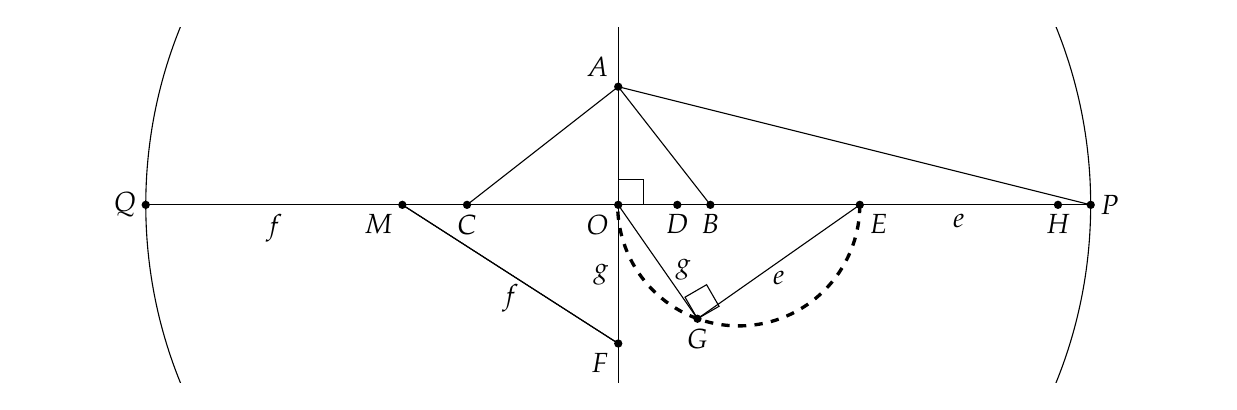
\begin{tikzpicture}[scale=1.5]
\clip (-5,-1.5) rectangle (5,1.5);
\coordinate (O) at (0,0);
\draw (O) circle (4cm);
\coordinate (P) at (4,0);
\coordinate (R) at (0,4);
\coordinate (Q) at (-4,0);
\coordinate (S) at (0,-4);
\coordinate (A) at (0,1);
\coordinate (B) at (.78,0);
\coordinate (C) at (-1.28,0);

\coordinate (D) at (.5,0);
\coordinate (E) at (2.045,0);
\coordinate (M) at (-1.8275,0);

\path[name path=circ] (M) circle (2.1725cm);
\path[name path=yaxis] (R) -- (S);
\path[name intersections={of=circ and yaxis,by={F1,F}}];
\draw (M) -- node[below] {$f$} (F);

\draw[name path=OEarc,very thick,dashed] (E) arc(0:-180:1.025cm);
\path[name path=OFcircle] (O)
  let
    \p1 = ($(O)-(F)$)
  in
    circle({veclen(\x1,\y1)});
\path[name intersections={of=OEarc and OFcircle, by={G}}];
\draw (O) -- node[above,near end,xshift=2pt] {$g$} (G) -- node[below] {$e$} (E);
\path (O) -- node[left] {$g$} (F);

\path[name path=EGcircle] (E) 
  let
  \p1 = ($(E)-(G)$)
  in
    circle({veclen(\x1,\y1)});
\draw[name path=PQ] (P) -- (Q);
\path[name intersections={of=PQ and EGcircle, by={H,H1}}];
\path (E) -- node[below] {$e$} (H);

\draw (R) -- (S);
\draw (A) -- (P);
\draw (C) -- (A) -- (B);
\draw (M) -- (F);

\foreach \c/\where in {O/below left, P/right, Q/left, R/above, S/below, A/above left, B/below, C/below, D/below, E/below right, M/below left, F/below left, G/below, H/below} {
  \fill (\c) circle(1pt) node[\where] {$\c$};
}
\draw (O) rectangle +(+6pt,+6pt);
\draw[rotate=30] (G) rectangle +(+6pt,+6pt);
\path (Q) -- node[below] {$f$} (M);
\end{tikzpicture}
\end{center}
\begin{form}{2}
\overline{OG}=\overline{OF}&=&\sqrt{\overline{MF}^2-\overline{MO}^2}=\sqrt{\overline{MF}^2-(1-\overline{MF})^2}\\
&=&\sqrt{2\overline{MF}-1}\\
&=&\sqrt{\disfrac{1}{16}\left(15-\sqrt{17}+\sqrt{34+2\sqrt{17}}\right)-1}\\
&=&\disfrac{1}{4}\sqrt{-1-\sqrt{17}+\sqrt{34+2\sqrt{17}}}\,.
\end{form}
$\angle OGE$ is a right angle since it is subtended by a diameter of the circle. Construct $H$ on $\overline{OP}$ such that $\overline{EH}=\overline{EG}$:
\begin{form}{2}
\overline{EH}=\overline{EG}&=&\sqrt{\overline{OE}^2-\overline{OG}^2}=\sqrt{(\overline{OB}+\overline{BE})^2-\overline{OG}^2}\\
&=&\sqrt{\left(\disfrac{-1+\sqrt{17}}{16}+\disfrac{\sqrt{34-2\sqrt{17}}}{16}\right)^2-
\disfrac{1}{16}\left(-1-\sqrt{17}+\sqrt{34+2\sqrt{17}}\right)}
\\
&=&\disfrac{1}{16}\sqrt{\left(
(18-2\sqrt{17})+ 2(-1+\sqrt{17})\sqrt{34-2\sqrt{17}}+
(34-2\sqrt{17})\right)+}\\
&&\quad\quad\quad\overline{
\left(16+16\sqrt{17}-16\sqrt{34+2\sqrt{17}}\right)}\\
&=&\disfrac{1}{16}\sqrt{
68+12\sqrt{17}-16\sqrt{34+2\sqrt{17}}-2(1-\sqrt{17})\sqrt{34-2\sqrt{17}}
}\,.
\end{form}
Let us compute $\overline{OE}$:
\begin{form}{2}
\overline{OE}=\overline{OB}+\overline{BE}&=&\disfrac{-1+\sqrt{17}}{16}+\disfrac{1}{16}\sqrt{34-2\sqrt{17}}\\
&=&\disfrac{1}{16}\left(-1+\sqrt{17}+\sqrt{34-2\sqrt{17}}\right)\,.
\end{form}
Finally, $\overline{OH}=\overline{OE}+\overline{EH}$ which is $\cos \left(\disfrac{2\pi}{17}\right)$.

%\end{comment}

\appendix
\section{Constructing an equilateral triangle}\label{a.triangle}

The central angle of an equilateral triangle is $360^\circ/3=120^\circ$ 
%(Figure~\ref{fig.triangle-pentagon}) 
and we can compute its cosine from the formula for the cosine of the sum of two angles:
\[
\cos 120^\circ = \cos(90^\circ+30^\circ)=\cos 90^\circ \cos 30^\circ  -\sin 90^\circ \sin 30^\circ = 0\cdot \frac{\sqrt{3}}{2} - 1\cdot \frac{1}{2}=-\disfrac{1}{2}\,.
\]
%\begin{figure}[htb]
\begin{center}
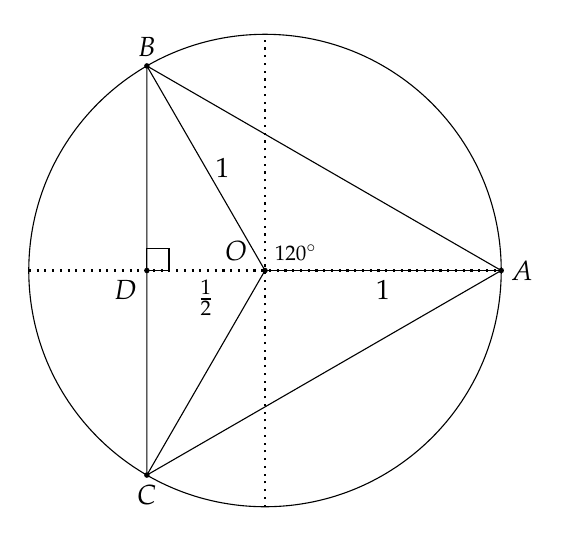
\begin{tikzpicture}[scale=1]
\coordinate (O) at (0,0);
\fill (O) circle(1pt);
\node[xshift=-3pt,above left] at (O) {$O$};
\foreach \x/\name/\pos in {0/A/right,1/B/above,2/C/below} {
  \coordinate (\name) at ($(O)+(\x*120:3cm)$);
  \draw (O) -- (\name) node[\pos] {$\name$};
  \fill (\name) circle (1pt);
}
\draw[thick,dotted] (-3,0) -- (3,0);
\draw[thick,dotted] (0,-3) -- (0,3);
\draw (A) -- (B) -- (C) -- cycle;
\node[above right] at (O) {\sm{120^\circ}};
\draw (O) circle (3cm);
\path (O) -- node[below] {$1$} (A);
\path (O) -- node[right] {$1$} (B);
\coordinate (D) at (-1.5,0);
\node[below left]  at (D) {$D$};
\fill (D) circle(1pt);
\path (O) -- node[below] {$\frac{1}{2}$} (D);
\draw (D) rectangle +(8pt,8pt);
\end{tikzpicture}
\end{center}
To construct the triangle, extend the radius $\overline{OA}$ of a unit circle to $D$ by the constructible length $\frac{1}{2}$. Construct the perpendicular throught $D$ that intersects the circle at $B,C$; then $\overline{AB},\overline{AC},\overline{BC}$ are the sides of an equilateral triangle inscribed in the unit circle. The side is $\overline{BD}+\overline{DC}$, which is:
\[
2\cdot \sqrt{1^2-\left(\disfrac{1}{2}\right)^2}=\sqrt{3}\,.
\]


\section{Constructing a regular pentagon}\label{a.pentagon}

\paragraph{The central angle of a regular pentagon}
The central angle is $360^\circ/5=72^\circ$. Let us compute $\cos 36^\circ$ using the  trigonometric identities for $2\theta$ and $\theta/2$ \cite{wiki:pentagon}:
\begin{form}{1.5}
0=\cos 90^\circ &=& \cos(72^\circ+18^\circ)\\
&=&(2\cos^2 36^\circ-1)\sqrt{\disfrac{1+\cos 36^\circ}{2}}-2\sin 36^\circ\cos 36^\circ\sqrt{\disfrac{1-\cos 36^\circ}{2}}\,.
\end{form}
There is now only one angle in the formula; let $x=\cos 36^\circ$. Then:
\begin{form}{1.5}
(2x^2-1)\sqrt{\disfrac{1+x}{2}}&=&2\sqrt{1-x^2}\cdot x \cdot \sqrt{\disfrac{1-x}{2}}\\
(2x^2-1)\sqrt{1+x}&=&2\sqrt{1-x}\cdot\sqrt{1+x}\cdot x \cdot \sqrt{1-x}\\
2x^2-1&=&2x(1-x)\\
4x^2-2x-1&=&0\,.
\end{form}
Solving the quadratic equation gives:
\[
\cos 36^\circ = \disfrac{1+\sqrt{5}}{4}\,,
\]
which can be computed using $\{+,-,\times,\div,\surd\}$ so it is constructible.

Figure~\ref{fig.pentagon} shows how to construct a regular pentagon from $\cos 36^\circ$. From $D$ at distance $\cos 36^\circ$ from $O$ construct a perpendicular to $\overline{OA}$ that intersects a unit circle at $C$. Construct $\overline{OC}$. Construct a line from $A$ perpendicular to $\overline{OC}$. Its intersection with the unit circle at $B$ defines $\overline{AB}$, the side of the inscribed pentagon. 

\begin{figure}[htb]
\begin{center}
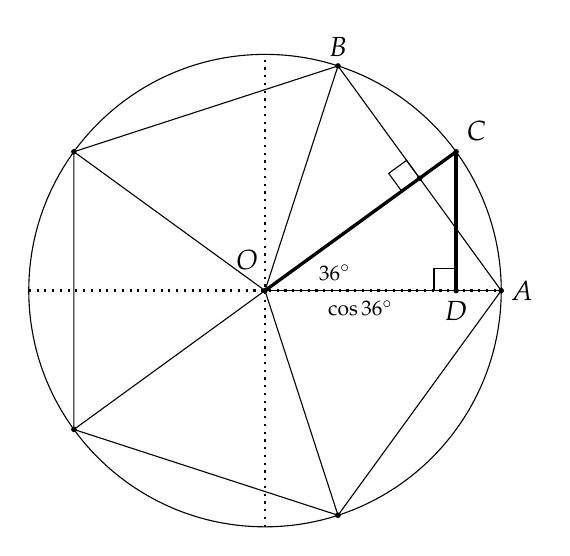
\begin{tikzpicture}[scale=1]
\coordinate (O) at (0,0);
\fill (O) circle(1pt) node[above left,xshift=1pt,yshift=4pt] {$O$};
\draw[thick,dotted] (-3,0) -- (3,0);
\draw[thick,dotted] (0,-3) -- (0,3);
\foreach \x/\name in {0/a,1/b,2/c,3/d,4/e} {
  \coordinate (\name) at ($(O)+(\x*72:3cm)$);
  \draw (O) -- (\name);
  \fill (\name) circle(1pt);
}
\draw (a) node[right] {$A$} -- (b) node[above] {$B$} -- (c) -- (d) -- (e) -- (a);
%\node[below right,xshift=4pt] at (O) {\sm{72^\circ}};
\node[above right,xshift=16pt] at (O) {\sm{36^\circ}};
\draw[very thick,name path=P1] (O) -- (36:3cm) coordinate (ten) node[above right] {$C$};
\path[name path=P2] (a) -- (b);
\path[name intersections={of=P1 and P2, by={right}}];
\coordinate (cos) at (ten|-a);
\draw[rotate=126] (right) rectangle +(8pt,8pt);
\draw[rotate=90] (cos) rectangle +(8pt,8pt);
\draw[very thick] (ten) -- (cos) node[below] {$D$};
\draw (O) circle (3cm);
\fill (right) circle (1pt);
\fill (ten) circle (1pt);
\fill (cos) circle(1pt);
\path (O) -- node[below] {\sm{\cos 36^\circ}} (cos);
\end{tikzpicture}
\caption{The central angle of a regular pentagon}\label{fig.pentagon}
\end{center}
\end{figure}

\paragraph{Direct construction of a regular pentagon}

Here is a solution to Exercises~2.3.3--2.3.4 of \cite[page~28]{stillwell}, 
showing that a regular pentagon is constructible.

Let $ABCDE$ be a regular pentagon whose sides are of length $1$. 

%\begin{figure}[htb]
\begin{center}
\begin{tikzpicture}[scale=.9]
\foreach \x/\name/\n/\po in {0/a/A/right,1/b/B/above,2/c/C/left,3/d/D/below left,4/e/E/below right} {
  \coordinate (\name) at ($(O)+(\x*72+18:3cm)$);
  \fill (\name) circle (1.5pt);
  \node[\po] at (\name) {$\n$};
}
\draw (a) -- (b) -- (c) -- node[left] {$1$} (d) -- node[below] {$1$} (e);
\draw[very thick] (e)-- node[right] {$1$} (a);
\draw[very thick] (a) -- (c);
\draw[very thick] (c) -- node[below] {$x$} (e);

\path[name path=ef] (e) -- +(108:5);
\path[name path=ac] (a) -- (c);
\path[name intersections={of=ac and ef,by={f}}];
\fill (f) circle(1.5pt);
\node[above] at (f) {$F$};
\draw[very thick] (e) -- node[right] {$1$} (f);
\path (a) -- node[above,xshift=-4pt] {$x-1$} (f);
\node[below left] at (a) {$\alpha$};
\node[below right,xshift=2pt] at (f) {$\alpha$};
\path (c) -- node[above] {$1$} (f);
\draw ($(e)+(72:.5)$) arc(72:144:.5cm);
\node[above,yshift=12pt] at (e) {$\alpha$};
\end{tikzpicture}
%\caption{Construction of a regular pentagon}\label{fig.pentagon1}
\end{center}
%\end{figure}
Construct the diagonals $\overline{AC}$ and $\overline{CE}$. $\angle AED=\angle EDC$ because they are the interior angles of a regular polygon. $\overline{AE}=\overline{CD}$ because they are the sides of a regular polygon. Therefore, $ACDE$ is an isoceles trapezoid and $\overline{AC}\parallel \overline{ED}$.


Construct a line through $E$ parallel to $\overline{DC}$ and let $F$ be its intersection with $\overline{AC}$. It follows that $\overline{EF}=1$.
Let $x$ be the length of the diagonals of the regular pentagon; it is easy to show that they are all equal. Then $\overline{AC}=\overline{CE}=x$, so $\triangle ACE$ is an isoceles triangle with base angles $\alpha$. $\triangle AEF$ is also isoceles so $\angle AFE=\angle FAE=\alpha$. Therefore, $\triangle ACE\sim\triangle AEF$:
\[
\disfrac{x}{1}=\disfrac{1}{x-1}\,.
\]
Multiplying out gives the quadratic equation:
\[
x^2-x-1=0\,,
\]
whose positive root is:
\[
\disfrac{1+\sqrt{5}}{2}\,.
\]
This length is constructible using rational numbers and square roots. The regular pentagon is constructible since from a line segment $\overline{AC}$ of length $\frac{1+\sqrt{5}}{2}$, construct the isoceles triangle $\triangle ABC$ which gives two sides and the interior angle of a regular pentagon.


\paragraph{Another demonstration that a regular pentagon is constructible}

Let $ABCDE$ be a regular pentagon whose sides are of length $1$.
%\begin{figure}[htb]
\begin{center}
\begin{tikzpicture}[scale=.9]
%\begin{scope}[xshift=7cm]
\foreach \x/\name/\n/\po in {0/a/A/right,1/b/B/above,2/c/C/left,3/d/D/below left,4/e/E/below right} {
  \coordinate (\name) at ($(O)+(\x*72+18:3cm)$);
  \fill (\name) circle (1.5pt);
  \node[\po] at (\name) {$\n$};
}
\draw (a) -- (b) -- (c) -- (d) -- node[below] {$1$} (e) -- node[right] {$1$} cycle;
\draw[name path=ac] (a) -- (c);
\path[name path=d] (d) -- ($(d)+(0,4)$);
\path[name path=e] (e) -- ($(e)+(0,4)$);
\path[name intersections={of=ac and d,by={f}}];
\fill (f) circle(1.5pt) node[above] {$F$};
\path[name intersections={of=ac and e,by={g}}];
\fill (g) circle(1.5pt) node[above] {$G$};
\draw[thick] (d) -- node[right] {$y$} (f);
\draw[thick] (e) -- node[left] {$y$} (g);
\draw[rotate=-90] (f) rectangle +(8pt,8pt);
\draw[rotate=-90] (g) rectangle +(8pt,8pt);
\draw[thick] (f) -- (a) -- (e);
\draw[thick] (a) -- node[below] {$x$} (d);
\draw[<->] ($(f)+(0,1)$) -- node[fill=white] {$1+\frac{x-1}{2}$} ($(a)+(0,1)$);
\path (f) -- node[above] {$1$} (g);
\end{tikzpicture}
%\caption{Construction of a regular pentagon}\label{fig.pentagon2}
\end{center}
%\end{figure}
Construct the diagonals $\overline{AD}= \overline{AC}$. Construct $\overline{DF} \perp \overline{AC}, \overline{EG}\perp \overline{AC}$. Let $y=\overline{DF}=\overline{EG}$.

By Pythagoras's theorem on $\triangle EGA, \triangle DFA$:
\begin{form}{1.8}
y^2+\left(\disfrac{x-1}{2}\right)^2&=&1^2\\
y^2+\left(1+\disfrac{x-1}{2}\right)^2&=&x^2\,.
\end{form}
Eliminate $y^2$ and simplify to obtain $x^2-x-1$. Continue as in the previous solution.

%\newpage
\bibliographystyle{plain}
\bibliography{heptadecagon}

\end{document}